 \chapter{Protocolo Experimental}
 \label{cap:protocoleo_experimental}
O preço de comutadores SDN baseados em \textit{OpenFLow} estão se tornando cada vez mais baratos com o passar dos anos, porém ainda possuem um custo elevado para elaboração de estudos em redes de larga escala, de modo que os emuladores ainda são os mais utilizados em experimentos, principalmente no meio acadêmico. O presente Capítulo tem o objetivo de apresentar a ferramenta gratuitas para criação e avaliação de cenários. A Seção \ref{sec:mininet}, apresenta um emulador que permite a criação de SDN baseadas no protocolo \textit{OpenFLow}. A Seção \ref{sec:aplicacao_teste_nas} apresenta uma aplicação baseada na comunicação MPI  para comparação das políticas. A Seção  \ref{sec:topologia} tem o objetivo de apresentar uma topologia de múltiplos caminhos, utilizada como cenário de teste. Por fim a Seção \ref{sec:metrica} estabelece a métrica necessária para o estudo.
 

\section{Emulador Mininet}
\label{sec:mininet}

\textit{Mininet} é uma emulador que permite criar uma rede virtual executando em um único computador ou MV através de comandos básicos para prototipação de redes tradicionais e SDN em larga escala. A ferramenta permite interagir de maneira fácil com a infraestrutura SDN por meio de uma interface de linha de comando (\textit{Command-line interface} (CLI)) e APIs, tornando-o frequentemente utilizado no desenvolvimento de pesquisas~\cite{mininet}. %CITAR MININET SITE

Por permitir a criação de uma infraestrutura com comutadores \textit{OpenFlow}, o \textit{Mininet} é uma ferramenta acessível para realização de casos de uso e comparação dos algoritmos de controle de fluxos. 
Por padrão o emulador possui quatro topologias básicas para realização de testes podendo ser facilmente alterada através de adição e remoção de servidores, comutadores, controladores e enlaces, que podem instanciados e adicionados a infraestrutura. Por se tratar de um emulador o controlador \textit{Floodlight} pode obter o controle de gerenciamento da rede virtual como se esta fosse um SDN físico, permitindo assim realizar as comparações das políticas de encaminhamento. 


%||||||||||||||||||||||||||||||||||||||||||||||||||||||||||||||||||||||||||||||||||||||||||
\subsection{Arquitetura}
\label{sub:arquiteturaMin}


Os principais componentes arquiteturais do \textit{Mininet} são detalhados a seguir~\cite{lantz2010network}.

\begin{itemize}
\item \textit{Enlaces}: Cria um par virtual que conecta um comutador a um computador permitindo assim o envio de pacotes de uma interface a outra. A classe ~\textit{TCLink} permite que seja definidos largura de banda e latência para os enlaces.

\item \textit{Computador:} No \textit{Mininet} um computador é um processo \textit{shell} no qual cada instancia pode possuir um processo isolado, com sua própria interface \textit{eth0}, sendo que a comunicação é isolada e só pode ser realizada entre esses processos pela de rede através dos enlaces.

\item \textit{Comutadores}: Os comutadores \textit{OpenFlow} do \textit{Mininet} oferecem a mesma semântica de encaminhamento de pacotes oferecido por um comutador \textit{OpenFlow} real, permitindo o gerenciamento por um controlador externo aderente ao padrão.
\item \textit{Controlador}:  O controlador pode ser executado tanto na rede virtual quanto externamente em um computador separado atreves de uma rede física.
\end{itemize}

Para auxiliar a criação de uma infraestrutura, o \textit{mininet} fornece uma API desenvolvida em ~\textit{Python}, e cada componente pode ser facilmente instanciado e adicionado a rede organizados de forma lógica para representar a uma rede real. 

%||||||||||||||||||||||||||||||||||||||||||||||||||||||||||||||||||||||||||||
\section{Aplicação para testes}
\label{sec:aplicacao_teste_nas}
Comparar e avaliar políticas de controle de fluxo é uma tarefa em que se considera o volume de tráfego transmitidos em um determinado intervalo de tempo. Levando em conta que a infraestrutura analisada não é uma infraestrutura física real, existem diversas barreiras que devem ser consideradas, tais como o escalonamento de processos do sistema operacional, infraestrutura, controlador e os processos utilizados para realizar troca de mensagens, que podem influenciar nos resultados.

Para essa avaliação foi utilizado o programa \emph{Numerical Aerodynamic Simulation} (NAS)~\cite{peterson1984numerical}, ferramenta que contém um conjunto de programas desenvolvidos pela \textit{National Aeronautics and Space Administration} (NASA), criados especificamente para avaliações de supercomputadores paralelos em diversos tamanhos de redes e \textit{grid} computacionais. Construído na linguagem de programação \textit{C}, esta ferramenta utiliza \emph{Message Passing Interface} (MPI) na construção de aplicações paralelas que trocam informações entre os servidores para a resolução de tarefas, sendo elas \emph{Block-Tridiagonal} (BT), \emph{Conjugate gradient} (CG), \emph{Embarrassingly parallel} (EP), \emph{Integer sort} (IS), \emph{Lower Upper} (LU), \emph{Multigrid} (MG) e \emph{Solution Pentadiagonal} (SP). 

\begin{figure}[!htb]
	\caption{\label{fig:padrao_nas}Padrão de comunicação da aplicação NAS em SDN.}
	\begin{center}
	    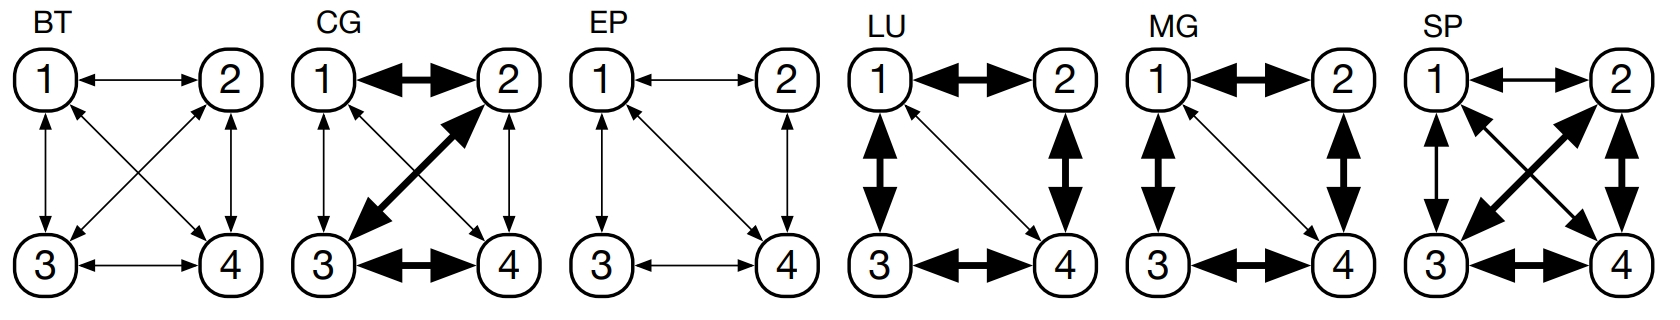
\includegraphics[scale=0.25]{imagens/padrao_comunicacao_nas.jpg}
	\end{center}
    \fonte{Elaborada por ~\cite{marcondes2016executing}.}	
\end{figure}

A figura \ref{fig:padrao_nas} ilustra o padrão de comunicação entre os processos separados em 4 servidores, na resolução de suas tarefas~\cite{marcondes2016executing}. A ilustração é um grafo em que cada vértice representa um servidor e as arestas representam o volume de dados trafegados entre os servidores. O volume de dados é representado pela largura das arestas, assim arestas finas representam pouca comunicação enquanto as mais largas representam maior comunicação. Nesse ambiente, ordenando as aplicações por volume de dados trafegados, EP necessita a troca de 10~KB para resolução de sua tarefa, a segunda menor aplicação BT necessita transmitir 48.04~MB, a terceira aplicação MG transfere 101.24~MB, CG transfere 137.23~MB, a aplicação LU 496.80~MB e a de maior volume de transferência é SP com 1,707.55~MB. O aumento da quantidade de servidores faz com que se aumente também a troca de informações devido à divisão da tarefa entre os processos MPI, porém as informações servem como base para se entender a diferença de desempenho das políticas em relação ao tempo de resoluções dos problemas.

%||||||||||||||||||||||||||||||||||||||||||||||||||||||||||||||||||||||||||||
\section{Topologia}
\label{sec:topologia}
A topologia escolhida para a análise dos algoritmos foi a \emph{Fat Tree}. Por se tratar de uma topologia comumente utilizada em alguns \emph{datacenters} contendo rotas alternativas e fornecendo maior escalabilidade. Criada com o auxílio da API \emph{python} do emulador \emph{Mininet}, essa topologia possui 3 camadas, a primeira chamada de núcleo, ligada com a segunda camada de agregação. A terceira camada possui os comutadores de arestas que são ligadas aos comutadores de agregação e os computadores da rede. \cite{alqahtani2018rethinking}. 
\begin{figure}[!htb]
	\caption{\label{fig:fattree}Design de uma \emph{Fat Tree} com \emph{4 POD.}}
	\begin{center}
	    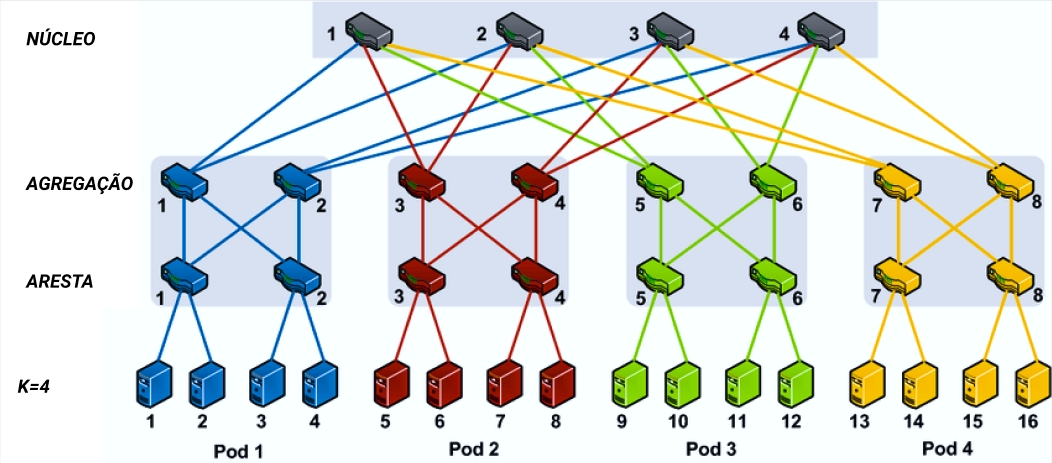
\includegraphics[scale=0.45]{imagens/fattree.jpg}
	\end{center}
    \fonte{Elaborada pelo autor (2021), baseado em \cite{al2008scalable}.}	
\end{figure}

Em uma \emph{Fat Tree}, \textit{k} representa a quantidade de PODs em que cada um deles possuem duas camadas de \textit{k/2} comutadores por camada. Cada \textit{k} quantidade de portas de um comutador da camada inferior (aresta) é dividida entre \textit{k/2} computadores e o restante das \textit{k/2} portas conectadas a camada superior de agregação. A primeira camada é o núcleo e  contém \textit{(k/2)²} comutadores sendo que cada uma das \textit{k} portas são conectadas a um POD diferente. Com isso, o número de POD é uma especificação que determina a relação entre portas e quantidade de comutadores. Por exemplo, com k=4, é obtido uma \emph{Fat Tree} com 4 POD, possuindo 4 comutadores por POD, em que cada comutador possui 4 portas divididas em dois \emph{uplinks} e 2 \emph{downlinks}. Ou seja, cada comutador de aresta possui 2 computadores em seus \emph{downlinks}, e dois comutadores de agregação em seus \emph{uplinks}. Os comutadores de núcleos possuem as 4 portas como \emph{downlinks} ligadas uma em cada POD \cite{al2008scalable}. A Figura \ref{fig:fattree} ilustra essa configuração de uma \emph{fattree} com 4 POD, dando um total de 16 computadores na rede. 

Essa topologia foi emulada em um computador com 4 GB de RAM e um processador intel core i3. Os enlaces são de \textit{1 GB/s} e 4 PODs foi o número máximo de maior estabilidade nas execuções dos programas do NAS. Cada um dos 16 servidores da \textit{Fat Tree} executam um \textit{daemond SSH} de modo a suportar as aplicações MPIs.

\section{Métrica Para Análise}
\label{sec:metrica}
Avaliar o desempenho de políticas de encaminhamento envolvendo diversos servidores é uma tarefa que pode considerar métricas como vazão, latência, perda de pacotes e tempo de resposta das requisições. Por exemplo, se for avaliar o \textit{download} de um servidor a outro, a eficiência dependeria do tráfego já existente na rede, e para isso seria necessário obter o mesmo tráfego para as diferentes políticas para que nenhuma seja prejudicada. Portanto, para facilitar foram definidas métricas em relação ao tempo que uma aplicação distribuída em vários servidores leva para solucionar um problema imutável. Assim ao executar essa mesma aplicação em diferentes políticas é encontrado tempos de execuções conforme a eficiência dos algoritmos de encaminhamento de fluxo.
Para isso o trabalho utilizou de várias aplicações do \textit{benchmark} NAS, cuja comunicação entre os servidores é crucial para a conclusão da tarefa. Ao término das execuções é obtido através de arquivos de \textit{log} o tempo que a tarefa levou para concluir. Sendo assim, foram feitas 10 execuções de cada aplicação do \textit{framework} para cada política apresentada. Os resultados obtidos foram agrupados para geração dos gráficos discutidos no Capítulo~\ref{cap:analise_resultados}.

\section{Considerações Parciais}
Este Capítulo fez uma revisão sobre o ambiente utilizado para comparação das políticas de encaminhamento de fluxo. Fez também a introdução a ferramenta \emph{Mininet}, usada para emular uma \emph{Fat Tree} \emph{OpenFlow} e introduziu a aplicação NAS, que por resolver tarefas que necessitam comunicações entre servidores tem sido utilizada em pesquisas acadêmicas, para avaliar computadores de alto desempenho em nuvens e \textit{clusters}. O Capítulo \ref{cap:analise_resultados} tem o intuito de fazer um estudo sobre os resultados obtidos pelas aplicações do NAS e comparar a eficiência das políticas implementadas.